%
%%%%%%%%%%%%%%%%%%%%%%%%%%%%%%%%%%%%%%%%%%%%%%%%%%
% PLANTILLA EJERCICIOS DE HISTORIA DE LA MÚSICA I
% Este es un modelo para redactar los ejercicios
% 
% Pasos para cubrir la plantilla:
% 1) Realizar una copia de este modelo
% 2) Renombrar el archivo:
%		"HM1_Hoja(número).tex"
% 3) El número de Hoja debe ser correlativo
% 
%%%%%%%%%%%%%%%%%%%%%%%%%%%%%%%%%%%%%%%%%%%%%%%%%%
%
% Esta plantilla es para crear ejercicios de esta materia
% Se recomienda crear un archivo por cada tema
% Descomentar según se necesite utilizar un modelo de ejercicio u otro
% Clase de documento:
\documentclass[letterpaper,12pt,notitlepage,spanish]{article}
%
% Archivo externo de configuración
% --------------------------------
% Seleccionar o idioma:
%%%%%%%%%%%%%%%%%%%%%%%%%%%%%%%%%%%%%%%%%%%
%% ---------- MODELO EJERCICIOS ---------- 
%% MATERIA: HISTORIA
%% CURSO: 
%% AÑO ACADÉMICO: 
%% CENTRO: 
%%%%%%%%%%%%%%%%%%%%%%%%%%%%%%%%%%%%%%%%%%%
%% 
%% MODELO PARA REDACTAR EJERCICIOS
%% ===============================
%% 
%% Clase de documento
%% ------------------
%\documentclass[letterpaper,12pt,notitlepage,spanish]{article}
%\documentclass[12pt,a4paper,notitlepage]{article}
%
% Márgenes de documento
% ---------------------
\usepackage[left=2.0cm, right=2.0cm, lines=45, top=2.5cm, bottom=2.0cm]{geometry}
%
% Paquetes necesarios
% -------------------
\usepackage[utf8]{inputenc} % acentos en ES
\usepackage[spanish,activeacute, es-tabla]{babel}
\usepackage{enumerate} % entornos de listas
\usepackage{multicol}  % varias columnas texto
\usepackage{fancyhdr}  % encabezado personalizado
\usepackage{fancybox}  % entornos con cajas
\usepackage{pdfpages}  % páginas pdf
%
\usepackage{lipsum} % generar texto aleatorio "loren ipsum"
\usepackage{environ} 
\usepackage{probsoln} % paquete para soluciones
%\showanswers % para mostrar soluciones
%
%Esto es lo importante. Ponemos la solución al margen.
\NewEnviron{solutionnew}{%
%  \leavevmode\marginpar{\raggedright\footnotesize \textbf{Solución:}\\ \BODY}
%  \textbf{Solución:}\\ \BODY} % sol. con salto de liña
  \small{Solución:} \BODY} % sol. na mesma liña
  {}
\renewenvironment{solution}{\solutionnew}{\endsolutionnew}
%
% FIGURAS EN COLUMNAS:
\newenvironment{Figura}
  {\par\medskip\noindent\minipage{\linewidth}}
  {\endminipage\par\medskip}
% ---
%
% Lineas de encabezado y pié
% --------------------------
\renewcommand{\headrulewidth}{0.5pt}
%\renewcommand{\headrulewidth}{1.0pt}
\renewcommand{\footrulewidth}{0.5pt}
%\renewcommand{\footrulewidth}{1.0pt}
\pagestyle{fancy} % estilo de página
%
% Recuadros y figuras
% -------------------
\newcommand\Loadedframemethod{TikZ}
\usepackage[framemethod=\Loadedframemethod]{mdframed}
\usepackage{tikz}
\usetikzlibrary{calc,through,backgrounds}
\usetikzlibrary{matrix,positioning}
%Desssins geometriques
\usetikzlibrary{arrows}
\usetikzlibrary{shapes.geometric}
\usetikzlibrary{datavisualization}
\usetikzlibrary{automata} % LATEX and plain TEX
\usetikzlibrary{shapes.multipart}
\usetikzlibrary{decorations.pathmorphing} 
\usepackage{pgfplots}
\usepackage{physics}
\usepackage{titletoc}
\usepackage{mathpazo} 
\usepackage{algpseudocode}
\usepackage{algorithmicx} 
\usepackage{bohr} 
\usepackage{xlop} 
\usepackage{bbding} 
%\usepackage{minibox} 
% Texto árabe
\usepackage{mathdesign}
\usepackage{bbding} 
% --
% Tipograía:
% ----------
% Fuente HEURÍSTICA (cómoda de leer)
%\usepackage{heuristica}
% Fuente LIBERTINE (cómoda para apuntes)
\usepackage{libertineRoman}
%\usepackage[proportional]{libertine}
% Fuente ROMANDE (estilo antiguo pero no muy cómoda)
%\usepackage{romande} %
% 
% Encabezado y pié de página (textos)
% -----------------------------------
% Modelo 1:
% ---------
% texto de encabezado izquierda:
%\lhead{\normalfont{Historia de la Música I}}
% texto encabezado centro:
%\chead{\textbf{Ejercicios}}
% texto de encabezado derecha:
%\rhead{\normalfont{curso: 2020/2021}}
% texto pié izquierdo:
%\lfoot{\small{\textit{}}}
% texto pié centrado:
%\cfoot{\textsc{Pág. \thepage }}
% texto pié derecho
%\rfoot{\textit{Pr. $\mathcal{A}$.Kaal}}
% ----------
% Modelo 2:
% ---------
% Encabezado y pié de página (textos)
% -----------------------------------
% texto de encabezado izquierda:
%
%\lhead{
%	\hrule
%	\vspace*{0.20cm}
%	\normalfont{Historia de la Música I}
%	\vspace*{0.10cm}
	%\hrule
%}
% texto encabezado centro:
%\chead{
%	\textbf{Cuestionario de Ejercicios}
%	\vspace*{0.08cm}}
% texto de encabezado derecha:
%\rhead{
%	\normalfont{curso: 2020/2021}
%	\vspace*{0.08cm}}
%
% texto pié izquierdo:
%\lfoot{
	%\begin{center}
		%\vspace*{0.20cm}
		%\hrule
		%\small{
		%Conservatorio Profesional de Música de Viveiro - Avda. da mariña s/n - (27850) Viveiro - Lugo
		%	}
	%\end{center}
%}
% texto pié centrado:
%\cfoot{
	%\vspace*{0.30cm}
	%\hrule
	%\vspace*{0.90cm}
%	\small{- Página \thepage -  }\\
	%\small{Conservatorio Profesional de Música de Viveiro}\\
	%\small{avda. da Mariña s/n}
%}

% ----------
% Modelo 3:
% ---------
% Encabezado y pié de página (textos)
% -----------------------------------
% texto de encabezado izquierda:
%
\lhead{
	\hrule
	\vspace*{0.20cm}
	\normalfont{Historia da Música I}
	\vspace*{0.10cm}
	%\hrule
}
% texto encabezado centro:
\chead{
	\textbf{CADERNO DE EXERCICIOS}
	\vspace*{0.08cm}}
% texto de encabezado derecha:
\rhead{
	\normalfont{curso: 2021/2022}
	\vspace*{0.08cm}}
%
% texto pié izquierdo:
%\lfoot{
	%\begin{center}
		%\vspace*{0.20cm}
		%\hrule
		%\small{
		%Conservatorio Profesional de Música de Viveiro - Avda. da mariña s/n - (27850) Viveiro - Lugo
		%	}
	%\end{center}
%}
% texto pié centrado:
\cfoot{
	%\vspace*{0.30cm}
	%\hrule
	%\vspace*{0.90cm}
	\small{- \thepage -  }\\
	%\small{Conservatorio Profesional de Música de Viveiro}\\
	%\small{avda. da Mariña s/n}
}

% --------
%=====================Algo setup
\algblock{If}{EndIf}
\algcblock[If]{If}{ElsIf}{EndIf}
\algcblock{If}{Else}{EndIf}
\algrenewtext{If}{\textbf{si}}
\algrenewtext{Else}{\textbf{sinon}}
\algrenewtext{EndIf}{\textbf{finsi}}
\algrenewtext{Then}{\textbf{alors}}
\algrenewtext{While}{\textbf{tant que}}
\algrenewtext{EndWhile}{\textbf{fin tant que}}
\algrenewtext{Repeat}{\textbf{r\'ep\'eter}}
\algrenewtext{Until}{\textbf{jusqu'\`a}}
\algcblockdefx[Strange]{If}{Eeee}{Oooo}
[1]{\textbf{Eeee} "#1"}
{\textbf{Wuuuups\dots}}

\algrenewcommand\algorithmicwhile{\textbf{TantQue}}
\algrenewcommand\algorithmicdo{\textbf{Faire}}
\algrenewcommand\algorithmicend{\textbf{Fin}}
\algrenewcommand\algorithmicrequire{\textbf{Variables}}
\algrenewcommand\algorithmicensure{\textbf{Constante}}% replace ensure by constante
\algblock[block]{Begin}{End}
\newcommand\algo[1]{\textbf{algorithme} #1;}
\newcommand\vars{\textbf{variables } }
\newcommand\consts{\textbf{constantes}}
\algrenewtext{Begin}{\textbf{debut}}
\algrenewtext{End}{\textbf{fin}}
%================================
%================================

\setlength{\parskip}{1.25cm}
\setlength{\parindent}{1.25cm}
\tikzstyle{titregris} =
[draw=gray,fill=gray, shading = exersicetitle, %
text=gray, rectangle, rounded corners, right,minimum height=.3cm]
\pgfdeclarehorizontalshading{exersicebackground}{100bp}
{color(0bp)=(green!40); color(100bp)=(black!5)}
\pgfdeclarehorizontalshading{exersicetitle}{100bp}
{color(0bp)=(red!40);color(100bp)=(black!5)}
\newcounter{exercise}
%\renewcommand*\theexercise{exercice \textbf{Ejercicio}~n\arabic{exercise}} % CASTELÁN
\renewcommand*\theexercise{exercice \textbf{Exercicio}~n\arabic{exercise}} % GALEGO
\makeatletter
\def\mdf@@exercisepoints{}%new mdframed key:
\define@key{mdf}{exercisepoints}{%
\def\mdf@@exercisepoints{#1}
}
\mdfdefinestyle{exercisestyle}{%
outerlinewidth=1em,outerlinecolor=white,%
leftmargin=-1em,rightmargin=-1em,%
middlelinewidth=0.5pt,roundcorner=3pt,linecolor=black,
apptotikzsetting={\tikzset{mdfbackground/.append style ={%
shading = exersicebackground}}},
innertopmargin=0.1\baselineskip,
skipabove={\dimexpr0.1\baselineskip+0\topskip\relax},
skipbelow={-0.1em},
needspace=0.5\baselineskip,
frametitlefont=\sffamily\bfseries,
settings={\global\stepcounter{exercise}},
singleextra={%
\node[titregris,xshift=0.5cm] at (P-|O) %
{~\mdf@frametitlefont{\theexercise}~};
\ifdefempty{\mdf@@exercisepoints}%
{}%
{\node[titregris,left,xshift=-1cm] at (P)%
{~\mdf@frametitlefont{\mdf@@exercisepoints points}~};}%
},
firstextra={%
\node[titregris,xshift=1cm] at (P-|O) %
{~\mdf@frametitlefont{\theexercise}~};
\ifdefempty{\mdf@@exercisepoints}%
{}%
{\node[titregris,left,xshift=-1cm] at (P)%
{~\mdf@frametitlefont{\mdf@@exercisepoints points}~};}%
},
}
\makeatother


%%%%%%%%%

%%%%%%%%%%%%%%%
\mdfdefinestyle{theoremstyle}{%
outerlinewidth=0.01em,linecolor=black,middlelinewidth=0.5pt,%
frametitlerule=true,roundcorner=2pt,%
apptotikzsetting={\tikzset{mfframetitlebackground/.append style={%
shade,left color=white, right color=blue!20}}},
frametitlerulecolor=black,innertopmargin=1\baselineskip,%green!60,
innerbottommargin=0.5\baselineskip,
frametitlerulewidth=0.1pt,
innertopmargin=0.7\topskip,skipabove={\dimexpr0.2\baselineskip+0.1\topskip\relax},
frametitleaboveskip=1pt,
frametitlebelowskip=1pt
}
\setlength{\parskip}{0mm}
\setlength{\parindent}{10mm}
%\mdtheorem[style=theoremstyle]{ejercicio}{\textbf{Ejercicio}} % Castelán
\mdtheorem[style=theoremstyle]{ejercicio}{\textbf{Exercicio}} % Galego
%================Liste definition--numList-and alphList=============
\newcounter{alphListCounter}
\newenvironment
{alphList}
{\begin{list}
{\alph{alphListCounter})}
{\usecounter{alphListCounter}
\setlength{\rightmargin}{0cm}
\setlength{\leftmargin}{0.5cm}
\setlength{\itemsep}{0.2cm}
\setlength{\partopsep}{0cm}
\setlength{\parsep}{0cm}}
}
{\end{list}}
\newcounter{numListCounter}
\newenvironment
{numList}
{\begin{list}
{\arabic{numListCounter})}
{\usecounter{numListCounter}
\setlength{\rightmargin}{0cm}
\setlength{\leftmargin}{0.5cm}
\setlength{\itemsep}{0cm}
\setlength{\partopsep}{0cm}
\setlength{\parsep}{0cm}}
}
{\end{list}}
%
%
%% -- Fin del archivo de configuración  --
%% % Galego
%\input{../../Modelos/include/config-HM1ejercicios_ES.tex} % Castelán
% --------------------------------
\usepackage{graphicx}
\usepackage{hyperref}
\begin{document}
%
% DATOS DE HOJA DE EJERCICIOS
% ---------------------------
%
% TÍTULO DE LA HOJA DE EJERCICIOS:
%
\begin{center}
\Large{
2º Trimestre
} \\
\vspace*{0.5cm}
%
% NÚMERO DE HOJA:
%
%\normalsize % Número de hoja:
%(XVII - XVIII)
%\\
\vspace{1.10cm}
	\begin{flushleft}
	Nome e Apelidos: \hrulefill\\
	%\vspace*{0.50cm}
%		\begin{center}
%		\small{Instrucciones para realizar los ejercicios}\\		
%		\end{center}
%	\hrulefill \\
	%\vspace*{0.25cm}
%
%\small{ % INSTRUCCIONES:
%\texttt{Lee con atención y realiza con detenimiento, los siguientes ejercicios teniendo en cuenta lo que se indica en cada uno. \\
%}} % fin instrucciones.
%
	\vspace*{0.25cm}		
 	\end{flushleft}
\end{center}
%
% ESPACIO PARA REDACTAR LOS EJERCICIOS:
% -------------------------------------  
%
% EXERCICIO 1.- Música en Grecia: transcrición epitafio Seikilos.
%
%% EXERCICIOS PARA INCLUÍR DENTRO DO CADERNO DE EXERCICIOS %%
%
% EXERCICIO DE TRANSCRICIÓN: Epitafio de Seikilos.
%
\section{Exercicio número 1}

Dentro das fontes conservadas da cultura musical grega, existen aproximadamente sobre uns vinte exemplos, malia que tan só uns poucos son considerados realmente fiables, en parte debido a que a maioría deles non se conservan na súa totalidade. 

O máis destacable é un fragmento da obra de \textit{Orestes}, de Eurípides do 250 a.C., aproximadamente. Trátase dun \textit{stasimon}, isto é, un coro cantado na \textit{orchestra} (lugar diante do escenario, onde se colocaban algúns dos participantes na traxedia). A conservación é realmente boa, a pesares de non ser perfecta debido a que foi escrito en papiro e algunhas das partes perdéronse.

\subsection*{O Epitafio de Seikilos}

A fonte de información da cultura grega de maior importancia que se conserva, e que máis información aporta, é o \textit{skolion} (epitafio) de Seikilos, do século II a.C. aproximadamente. Escrito en pedra (nunha estela funeraria da actual Turquía conservado en Dinamarca), presenta unha magnífica conservación que permitiu descifralo totalmente. Podemos afirmar que é a obra máis coñecida da Antiga Grecia.

\subsubsection*{O texto}

Inscrita nunha columna (estela funeraria), serviu de epitafio a unha muller: na dedicatoria, Seikilos ofrece a unha muller (probablemente a súa esposa ou filla) unha canción, que aparece con notación musical e texto:

\begin{figure}[htp]
\centering
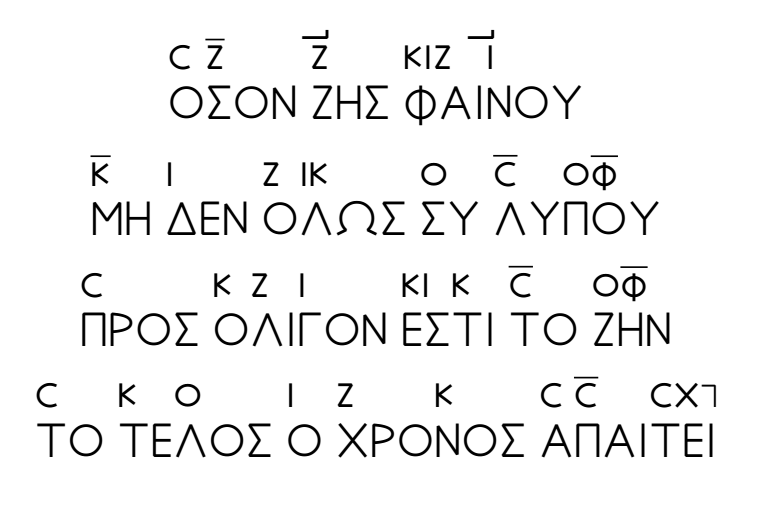
\includegraphics[scale=1.00]{images/Seikilos-Ejercicio-03.png}
\caption{Texto do epitafio de Seikilos}
\label{Seikilos-texto}
\end{figure}

A tradución sería algo semellante a: \textit{ Mentres vivas, brilla; que nada te faga sufrir; a vida é moi curta e o tempo marca a fin.}

A achega máis destacable ou importante deste documento histórico aos estudos da música grega, foi sen dúbida a notación rítmica, que ao igual que a melódica, emprega signos do alfabeto grego. As notas sen indicación rítmica, valerían un pulso (\textit{chronos protos}), as sinaladas cun guión terían dous pulsos (\textit{diseme}); finalmente, as que levan guión cun sinal ou punto na parte superior dereita valerían tres pulsos (*\textit{triseme}).

\subsubsection*{A notación musical}

\begin{itemize}
\item Para indicar a altura dos sons, empregábase un signo diferente segundo cada altura. Os signos que aparecen nesta peza, ordenados de xeito ascendente son:

	\begin{figure}[htp]
	\centering
	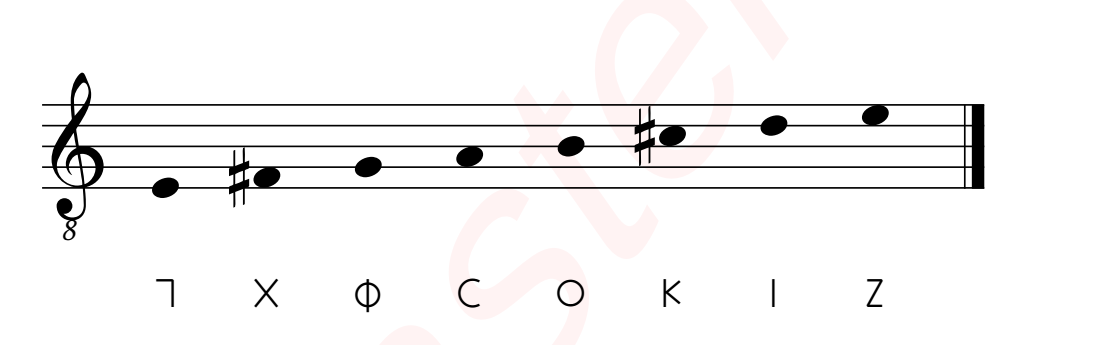
\includegraphics[scale=1.00]{images/Seikilos-Ejercicio-01.png}
	\caption{Sitema de notación}
	\label{seikilos-sistema}
	\end{figure}
	
\item Para indicar a duración, empregábanse uns signos adicionais sobre os anteriores:
	\begin{figure}[htp]
	\centering
	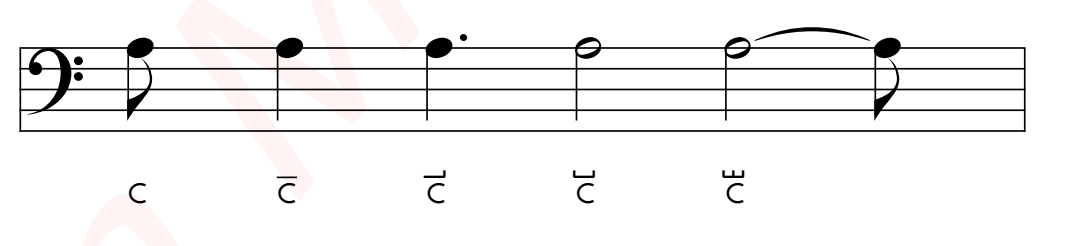
\includegraphics[scale=1.00]{images/Seikilos-Ejercicio-02.png}
	\caption{Indicación da duración}
	\label{seikilos-duracion}
	\end{figure}
	
\end{itemize}

\subsubsection*{Transcrición}

Tendo en conta o indicado ata o de agora, realiza unha transcrición á notación actual da melodía do epitafio de Seikilos.

\begin{figure}[htp]
\centering
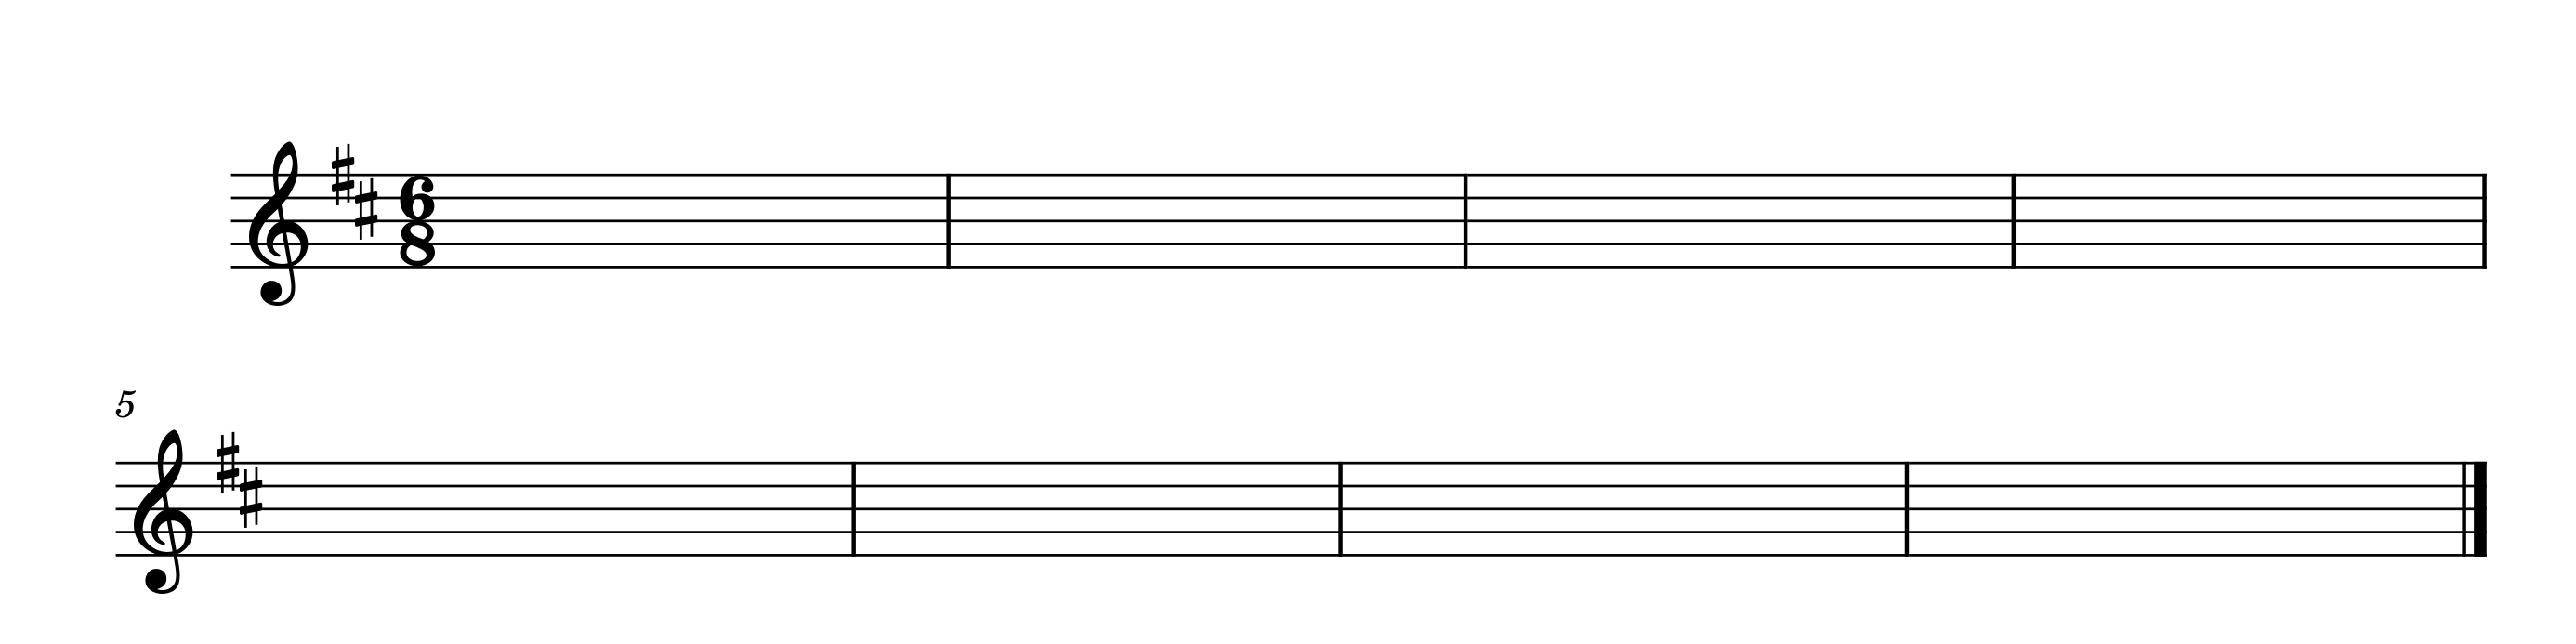
\includegraphics[scale=0.90]{images/Seikilos-1.png}
\caption{Transcrición a notación moderna do epitadio de Seikilos}
\label{transcricion}
\end{figure}

\newpage
%
% EXERCICIO 2.- Música na antigüidade clásica
%
%% EXERCICIOS PARA INCLUÍR DENTRO DO CADERNO DE EXERCICIOS %%
%
% EXERCICIO.- 
%
\section{A música na antigüidade clásica}
%
% Pequena introdución ás audicións
%
Dentro das audicións incluídas no tema da música en Grecia, escoitaremos entre outras, o \textit{Epitafio de Seikilos} do exercicio anterior. 
Tanto para esta, como para as que escoitemos ao longo do curso, convén ter en conta tanto os elementos externos (instrumentos e intérpretes), como os internos (forma, xénero, estilo) da propia música. 
Debemos tomar notas e realiar para nós mesmos, un pequeno comentario-análise; hai que ter en conta que non se trata de oír simplemente, senón de escoitar os matices da música.
%
\subsection*{Elementos mínimos a ter en conta nunha audición}
%
%\begin{enumerate}[1.-]
%PUNTO NÚMERO 1: ESCOITAR A PEZA
%
Debemos ter en conta, que para comprender a música das diferentes épocas ou períodos da historia, precisamos escoitala: un dos obxectivos de realizar audicións, é precisamente ese. 
Como plantexamos, xa que logo as audicións?
\par
Trátase de escoitar a peza completa con atención; non importa, se non a identificamos á primeira. Anotaremos as cuestións musicais básicas, como:
%
%\begin{multicols}{2}
%
    \begin{enumerate}[1.-]
        %
        \item % TIMBRE
        \textbf{Timbre}: identificamos os instrumentos e voces que interveñen, prestando atención en cales teñen máis relevancia. Se non coñecemos ben algún timbre podemos determinar a familia instrumental á que pertence (cordófono, aerófono, membranófono, idiófono).
        \par %Pregunta sobre o timbre
        - Que timbres recoñeces na audición? \dotfill
        \par % Consello:
        Se non recoñeces algún, podes anotar aquelas características que escoitas, para tentar identificalo posteriormente.
        %
 %
        \item %MELODÍA:
        \textbf{Melodía}: debemos fixarnos e indicar como son as melodías, partindo de cuestións do tipo: 
        \begin{multicols}{2}
        \begin{itemize}
            \item 
            Son longas ou curtas? \dotfill
            \item 
            Que figuras empregan? \dotfill
            \item
            Cal é o seu ámbito? \dotfill
            \item
            Móvense por graos conxuntos ou por saltos? \dotfill
            \item
            Que perfil teñen (ascendente, descendente, en arco, etc.)? \dotfill
            \item
            Repítese a melodía? Cantas veces? \dotfill
            \item
            Que instrumentos levan as melodías principais? \dotfill
        \end{itemize}
        \end{multicols}
%
        \item %TEXTURA
        \textbf{Textura}: prestaremos atención a como se ensamblan as diferentes voces:
            \begin{enumerate}[a)]
                \item Texturas melódicas: 
                \begin{itemize}
                    \item
                    De escrita horizontal: 
                    \begin{itemize}
                        \item 
                        \textbf{textura monódica}: unha única liña melódica onde todos interpretan o mesmo
                        \item
                        \textbf{textura polifónica}: varias liñas melódicas interpretadas todas á vez   
                    \end{itemize}
                    \item
                    De escrita vertical: 
                    \begin{itemize}
                        \item 
                        \textbf{textura homofónica} ou \textbf{harmónica}: unha melodía principal acompañada por acordes
                    \end{itemize}
                \end{itemize}
                \item
                Texturas non melódicas
            \end{enumerate}
            \par %Pregunta sobre a textura
            - Que tipo de textura recoñeces na audición? \dotfill
            \par % Consello:
            Presta atención ao que escoitas e indica se so hai melodía, melodía con acompañamento, que fai o acompañamento en relación á melodía principal, (...).
%
        \item % RITMO:
        \textbf{Ritmo}: identificaremos o comportamento da rítmica dentro da peza que escoitemos.
        \begin{itemize}
            \item 
            Hai ritmo constante ou cambiante? \dotfill
            \item
            É rápido, lento, marcado, libre, (...)? \dotfill
            \item
            Identificas algún compás (división, subdivisión, (...)? \dotfill
            \item
            Escoitas algunha voz leva o ritmo? Cal? \dotfill
        \end{itemize}
%
        \item % HARMONÍA:
        \textbf{Harmonía}: identificaremos, no caso de texturas homofónicas, tonalidade, modalidade, atonalidade. No caso de pezas polifonía, hai que fixarse tamén no uso de consonancias ou disonancias.
        \par %Pregunta sobre a textura
        - Segundo a textura da peza, podemos dicir que hai algún tipo de acompañamento harmónico? \dotfill
%
        \item %FORMA:
        \textbf{Forma}: despois de escoitar a peza completa, farémonos unha idea dos instrumentos, da extensión (duración) que ten e tamén da estrutura. Debemos identificar aquí, se é o caso, cales son as partes (seccións, movementos, ...) da obra ou peza e que trazos ten cada unha delas. Dentro dos tipos de formas que debemos coñecer, identificaremos:
            \begin{enumerate}[a)]
                \item
                Segundo a extensión:
                \begin{itemize}
                    \item
                    \textbf{Formas maiores}, de diferentes movementos ou grandes dimensións
                    \item
                    \textbf{Formas menores}, un só movemento ou de curta duración
                \end{itemize}
                \item
                Segundo os instrumentos ou voces:
                 \begin{itemize}
                    \item
                    \textbf{Formas vocais}, con intervención da voz humana
                    \item
                    \textbf{Formas instrumentais}, só instrumentos
                \end{itemize}
                \item 
                Segundo a súa estrutura:
                \begin{itemize}
                    \item 
                    \textbf{Formas estruturadas}, ou fixas: aquelas con esquema compositivo determinado, como por exemplo sonatas, sinfonías, etc.
                    \item
                    \textbf{Formas libres}: non respetan aparentemente ningunha estrutura definida
                \end{itemize}
            \end{enumerate}
        \par %Pregunta sobre as Formas
        - A que tipo de forma, podemos dicir que se axusta a peza? \dotfill
        \par % Consello:
        Ten en conta, que ata o momento estamos a escoitar pequenas pezas onde se combina a voz con certos instrumentos e malia que pode semellar que non teñen un esquema compositivo fixo, pode dar lugar a confusión.    
        \end{enumerate}
%    \end{multicols}
%
\subsubsection*{Notas sobre a audición}
Redacta un breve comentario sobre a audicióno que acabamos de escoitar tendo en conta os puntos anteriores.
%
\begin{ejercicio}[Comentario resumo do \textit{Epitafio de Seikilos}]
% ESPACIO PARA REDACTAR O COMENTARIO DA AUDICIÓN
        \vspace*{2.78cm}
\end{ejercicio}
%
% --------------------------
% EXPLICACIÓN DAS AUDICIÓNS:
% --------------------------
%
%\newpage
%
%\subsection*{Recoñecemento auditivo de formas vocais e instrumentais}
%
%Escoita con atención as dúas obras que se propoñen como exercicios de audición e completa as fichas correspondentes. Procura información sobre as mesmas e sobre o autor para coñecer o seu contexto.
%\par
%\begin{multicols}{2}
%
% AUDICIÓN 3.- HIMNO A NÉMESIS
% ----------------------------
% Suite "Música acuática" de George Friedrich Haendel (1685-1759)
%
%\begin{ejercicio}[]
%
%Completa a ficha da obra proposta como exercicio de audición.
%
%	\begin{enumerate}[1.-]
%        \vspace*{0.3cm}
%		\item
%			Autor: \dotfill
%			\vspace*{0.3cm}
%		\item
%			Obra:
%			\begin{enumerate}[a)]
%			    \item Título: \dotfill \vspace*{0.3cm}
%			    \item Forma: \dotfill \vspace*{0.3cm}
%			    \item Xénero: \dotfill \vspace*{0.3cm}
%			    \item Estilo: \dotfill \vspace*{0.3cm}
%			    \item Instrumentación: \dotfill 
%			    \vspace*{0.3cm}
%			\end{enumerate}
%		\item 
%		    Resume as principais características que definen a obra:
%			\vspace*{10.0cm}			
%
%	\end{enumerate}
%\end{ejercicio}
%
% AUDICIÓN 4.- EPITAFIO SEIKILOS
% --------------------------------------------
% Oratorio "El Mesías" de George Friedrich Haendel (1685-1759)
%
%\begin{ejercicio}[]
%
%Completa a ficha da obra proposta como exercicio de audición.
%
%	\begin{enumerate}[1.-]
%        \vspace*{0.3cm}
%		\item
%			Autor: \dotfill
%			\vspace*{0.3cm}
%		\item
%			Obra:
%			\begin{enumerate}[a)]
%			    \item Título: \dotfill \vspace*{0.3cm}
%			    \item Forma: \dotfill \vspace*{0.3cm}
%			    \item Xénero: \dotfill \vspace*{0.3cm}
%			    \item Estilo: \dotfill \vspace*{0.3cm}
%			    \item Instrumentación: \dotfill 
%			    \vspace*{0.3cm}
%			\end{enumerate}
%		\item 
%		    Resume as principais características da obra:
%			\vspace*{10.0cm}			
%
%	\end{enumerate}
%\end{ejercicio}
%
%\end{multicols}
%
%\newpage
%
%
%\begin{multicols}{2}
%
% AUDICIÓN 3.- HIMNO A NÉMESIS
% ----------------------------
% Suite "Música acuática" de George Friedrich Haendel (1685-1759)
%
%\begin{ejercicio}[]
%
%Completa a ficha da obra proposta como exercicio de audición.
%
%	\begin{enumerate}[1.-]
%        \vspace*{0.3cm}
%		\item
%			Autor: \dotfill
%			\vspace*{0.3cm}
%		\item
%			Obra:
%			\begin{enumerate}[a)]
%			    \item Título: \dotfill \vspace*{0.3cm}
%			    \item Forma: \dotfill \vspace*{0.3cm}
%			    \item Xénero: \dotfill \vspace*{0.3cm}
%			    \item Estilo: \dotfill \vspace*{0.3cm}
%			    \item Instrumentación: \dotfill 
%			    \vspace*{0.3cm}
%			\end{enumerate}
%		\item 
%		    Resume as principais características que definen a obra:
%			\vspace*{13.0cm}			
%
%	\end{enumerate}
%\end{ejercicio}
%
% AUDICIÓN 4.- EPITAFIO SEIKILOS
% --------------------------------------------
% Oratorio "El Mesías" de George Friedrich Haendel (1685-1759)
%
%\begin{ejercicio}[]
%
%Completa a ficha da obra proposta como exercicio de audición.
%
%	\begin{enumerate}[1.-]
%        \vspace*{0.3cm}
%		\item
%			Autor: \dotfill
%			\vspace*{0.3cm}
%		\item
%			Obra:
%			\begin{enumerate}[a)]
%			    \item Título: \dotfill \vspace*{0.3cm}
%			    \item Forma: \dotfill \vspace*{0.3cm}
%			    \item Xénero: \dotfill \vspace*{0.3cm}
%			    \item Estilo: \dotfill \vspace*{0.3cm}
%			    \item Instrumentación: \dotfill 
%			    \vspace*{0.3cm}
%			\end{enumerate}
%		\item 
%		    Resume as principais características da obra:
%			\vspace*{13.0cm}			
%
%	\end{enumerate}
%\end{ejercicio}
%
%\end{multicols}
%
\newpage
%
% EXERCICIO 3.- Teoría musical
%
%
% Repaso de conceptos de teoría musical grega
\section{A música en Grecia}
%
Para escoitar e comprender ben a música dos diferentes períodos da cultura grega, debemos coñecer as principais características ou trazos que a definen. Coñecer as características, axuda a diferenciar a música de diferentes culturas, épocas, civilizacións e, asimesmo, será de utilidade á hora de completar a ficha de audición. Repasaremos aquí os aspectos básicos.
%
\subsection*{Fundamentos da teoría musical grega}\label{fundamentos}
%
Le con atención as características que definen os fundamentos da teoría musical grega e trata de identificalos nas audicións.
\begin{multicols}{2}
    \begin{enumerate}[1)]
    \item
    A música grega era \textbf{principalmente monódica}: o acompañamento instrumental, non implica harmonía ou polifonía na música grega
    \item
    Empregaba \textbf{notación alfabética}:  diferente segundo se tratase de música vocal ou instrumental
    \item
    Inicialmente emprega \textbf{ritmo libre} axustado á prosodia do texto; música e verso van unidos. Posteriormente, aparecen os \textbf{pés métricos} que se basan na duración longa ou curta das sílabas, sendo os máis comúns: \textit{Yambo}, \textit{Troqueo}, \textit{Anapesto}, \textit{Dáctilo}, (...)
    \item
    Emprega \textbf{Métrica} rica e complicada
    \item
    A \textbf{melodía} responde á idea do \textit{nomos} (lei), semellante a unha especie de patrón, esquema ou norma que rixe o sistema de composición
    \item
    O sistema musical grego é \textbf{modal}, baseado no uso do \textit{tetracordo} descendente de 4 notas
    \item
    Os \textbf{modos gregos}, están definidos polos \textit{tetracordos} e segundo a posición destes reciben un nome ou outro, que ven definido pola colocación dos \textit{semitonos} (e a súa relación interválica) e non polas notas que empregan. Os principais son:
        \begin{itemize}
            \item
            \textit{tetracordo} \textit{dórico} (T T S) = \textbf{modo dórico}, corresponde á oitava Mi-Mi
            \item
            \textit{tetracordo} \textit{frixio} (T S T) = \textbf{modo frixio}, corresponde á oitava Re-Re
            \item
            \textit{tetracordo} \textit{lidio} (S T T) = \textbf{modo lidio}, corresponde á oitava Dó-Dó
            \item
            \textbf{Modo mixolidio}, non emprega dous \textit{tetracordos} iguais = oitava Si-Si
        \end{itemize}
    \item
    Os sons a partir dos cales se organiza o sistema musical grego, parten de relacións numéricas sinxelas definidas por Pitágoras a partir do \textit{monocordio}
    \item
    O sistema musical grego, recibe o nome de \textbf{\textit{sistema diatónico teleion}} que comprende 2 oitavas.
    \item
    A escala Mi-Mi é a máis importante: coincide coa afinación (das cordas) da \textit{kithara} e coñecíase tamén co nome de "Harmonía"
    \end{enumerate}
\end{multicols}
%
\subsection*{Os tres himnos de Mesomedes de Creta}
%
Escoita os tres himnos de Mesomedes de Creta (\textit{Invocación a Calíope e Apolo}, \textit{Himno a Helio} e \textit{Himno a Némesis}) que podes atopar na {\href{https://open.spotify.com/playlist/19fWZwUGX6rDo0bejNcWGE?si=1c00d5ff65b24678}{\textcolor{blue}{lista de audicións}}} de Spotify e trata de identificar as principais características da teoría musical grega que se indican no punto anterior.
\par
%
\subsubsection*{O \textit{Himno a Némesis}}
%
Este himno de Mesomedes de Creta, é un dos catro que conservan notación musical antiga sobre o texto; a figura \ref{nemesis-himno} é unha transcrición a notación actual do himno.
%
\begin{figure}[htp]
    \centering
	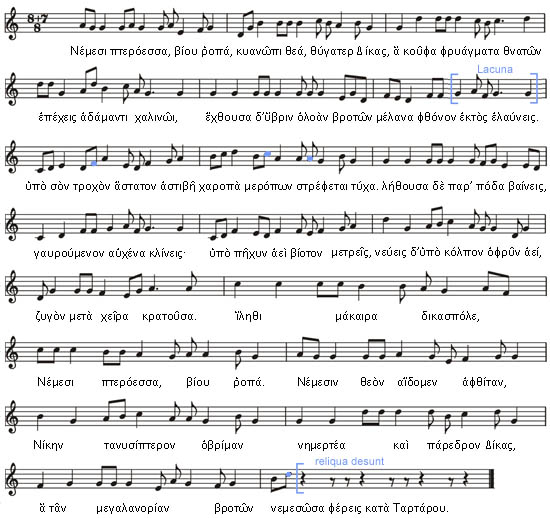
\includegraphics[scale=0.80]{images/mes-hnem.jpg}
	\caption{Exemplo do himno a némesis}
	\label{nemesis-himno}
	\end{figure}
%
\begin{ejercicio}[Comentario resumo do \textit{Himno a Némesis}]
Fai un breve comentario sobre o himno, seguindo os puntos anteriores.
% ESPACIO PARA REDACTAR O COMENTARIO DA AUDICIÓN
        \vspace*{3.3cm}
\end{ejercicio}
 

\newpage
%


% EXERCICIO PARA AUDICIÓN HIMNO A NÉMESIS
%
\begin{ejercicio}[Audición \textit{Himno a Némesis}]
%
Atendendo aos elementos mínimos que debes ter en conta para elaborar un comentario de audición (indicados no punto 2 do caderno de exercicios), completa a seguinte ficha.
%
    \begin{enumerate}[1.-]
    \item \textbf{Autor.} Indica o autor da obra (se é posible) \dotfill
    \item \textbf{Título da obra.} Indica o título da obra \dotfill
%    \begin{multicols}{2}
        \item 
        \textbf{Timbre.}
%        \begin{enumerate}
%        \item 
        Indica os instrumentos que recoñeces na audición, segundo a clasificación moderna.
        \vspace*{1.0cm}
%            \begin{enumerate}
%            \item Cordófonos \dotfill
%            \item Aerófonos \dotfill
%            \item Idiófonos \dotfill
%            \item Membranófonos\dotfill
%            \item Outros \dotfill
%            \end{enumerate}
%        \end{enumerate}
%    \end{multicols}
%
        \item
        \textbf{Textura.}
        Estamos ante textura de escrita horizontal ou vertical? \dotfill
        \par
        Cal é, das que coñeces? (homofonía, polifonía, monodia, etc.) \dotfill \par
%
        \item
        \textbf{Melodía.}
            Para determinar a textura, fíxate na melodía prestando atención a:
            \begin{enumerate}
            \item Que son é o son que máis se repite? \dotfill
            \item Por que ámbito se move? (2as, 3as, grandes saltos, ...) \dotfill
            \item Que fan os instrumentos con respecto á voz? \dotfill
            \item Cantos instrumentos identificas de cada familia? \dotfill
            \item Algún dos instrumentos leva a voz principal? Se é así, cal(es)?\dotfill
        \end{enumerate}
        \item 
        \textbf{Ritmo.}
        \begin{enumerate}
            \item
            Identifica as figuras e trata de establecer o tempo (pulso, compás) en caso de que non se indique.
            \begin{enumerate}
                \item Que figuras identificas? \dotfill
                \item Identificas un tempo longo, breve, ...? \dotfill
                \item Podemos identificar o compás? 
                \item Se é o caso, cal? \dotfill
            \end{enumerate}
            \item 
            Atendento á rítmica, presta atención aos seguintes aspectos:
            \begin{enumerate}
                \item É ritmo constante ou cambiante? \dotfill
                \item Podemos dicir que é rápido ou lento? \dotfill
                \item Estamos ante un ritmo libre? \dotfill
                \item Quen leva o ritmo? (voz, instrumentos de vento, ...) \dotfill
            \end{enumerate}
        \end{enumerate}
        \item 
        \textbf{Forma.}
        Determina segundo a extensión, instrumentación e estrutura da obra, a forma:
        \begin{enumerate}
            \item Estamos ante unha forma maior ou menor? \dotfill
            \item O timbre fainos pensar que se trata de unha forma? \dotfill
            \item Estamos ante unha forma libre? Por que? \dotfill
        \end{enumerate}
    \end{enumerate}
%
\end{ejercicio}
%
% EXERCICIO PARA AUDICIÓN EPITAFIO SEIKILOS
%
\begin{ejercicio}[Audición \textit{Epitafio de Seikilos}]
%
Atendendo aos elementos mínimos que debes ter en conta para elaborar un comentario de audición (indicados no punto 2 do caderno de exercicios), completa a seguinte ficha.
%
    \begin{enumerate}[1.-]
    \item \textbf{Autor.} Indica o autor da obra (se é posible) \dotfill
    \item \textbf{Título da obra.} Indica o título da obra \dotfill
%    \begin{multicols}{2}
        \item 
        \textbf{Timbre.}
%        \begin{enumerate}
%        \item 
        Indica os instrumentos que recoñeces na audición, segundo a clasificación moderna.
        \vspace*{1.0cm}
%            \begin{enumerate}
%            \item Cordófonos \dotfill
%            \item Aerófonos \dotfill
%            \item Idiófonos \dotfill
%            \item Membranófonos\dotfill
%            \item Outros \dotfill
%            \end{enumerate}
%        \end{enumerate}
%    \end{multicols}
%
        \item
        \textbf{Textura.}
        Estamos ante textura de escrita horizontal ou vertical? \dotfill
        \par
        Cal é, das que coñeces? (homofonía, polifonía, monodia, etc.) \dotfill \par
%
        \item
        \textbf{Melodía.}
            Para determinar a textura, fíxate na melodía prestando atención a:
            \begin{enumerate}
            \item Que son é o son que máis se repite? \dotfill
            \item Por que ámbito se move? (2as, 3as, grandes saltos, ...) \dotfill
            \item Que fan os instrumentos con respecto á voz? \dotfill
            \item Cantos instrumentos identificas de cada familia? \dotfill
            \item Algún dos instrumentos leva a voz principal? Se é así, cal(es)?\dotfill
        \end{enumerate}
        \item 
        \textbf{Ritmo.}
        \begin{enumerate}
            \item
            Identifica as figuras e trata de establecer o tempo (pulso, compás) en caso de que non se indique.
            \begin{enumerate}
                \item Que figuras identificas? \dotfill
                \item Identificas un tempo longo, breve, ...? \dotfill
                \item Podemos identificar o compás? 
                \item Se é o caso, cal? \dotfill
            \end{enumerate}
            \item 
            Atendento á rítmica, presta atención aos seguintes aspectos:
            \begin{enumerate}
                \item É ritmo constante ou cambiante? \dotfill
                \item Podemos dicir que é rápido ou lento? \dotfill
                \item Estamos ante un ritmo libre? \dotfill
                \item Quen leva o ritmo? (voz, instrumentos de vento, ...) \dotfill
            \end{enumerate}
        \end{enumerate}
        \item 
        \textbf{Forma.}
        Determina segundo a extensión, instrumentación e estrutura da obra, a forma:
        \begin{enumerate}
            \item Estamos ante unha forma maior ou menor? \dotfill
            \item O timbre fainos pensar que se trata de unha forma? \dotfill
            \item Estamos ante unha forma libre? Por que? \dotfill
        \end{enumerate}
    \end{enumerate}
%
\end{ejercicio}
%
\begin{ejercicio}[Audición comentada \textit{Epitafio Seikilos}]
Le con atención a seguinte audición comentada do \textit{Epitafio de Seikilos}, fixándote nos diferentes aspectos que se comentan.
%
   \begin{enumerate}[1.-]

       \item \textbf{Contextualización}
       \par
O Epitafio de Seikilos é un fragmento de inscrición epigráfica grega achado nunha columna de mármore posta sobre a tumba que fixera construír Seikilos para a súa esposa Euterpe, preto de Trales (en Asia Menor).
\par
Conservada actualmente no Museo Nacional de Dinamarca, foi descuberta en 1883 por Sir W. M. Ramsay en Turquía e conservada no museo da antiga cidade de Esmirna. Durante o holocausto de Asia Menor (1919-1922), no que a cidade de Esmirna foi destruida, non se tivo coñecemento do seu paradeiro; posteriormente foi recuperada con sinais de desgaste e deterioro na súa base e coa última liña do texto borrada.
\par
Este manuscrito constitúe un exemplo de forma de composición musical grega, co engadido de ser a melodía escrita máis antiga que se coñece. A inscrición, contén un texto en grego sobre o que se desenvolve a melodía

   \item \textbf{Timbre} \par
A canción é melancólica, clasificada como \textit{skolion} ou "canción para beber".

    \item \textbf{Textura} \par
    \begin{itemize}
        \item 
        A composición está construída e organizada segundo principios modais.
        \item 
        Está en modo *Mixolidio actual e desenvólvese nun ámbito de oitava xusta. 
        \item
        Aparecen todos os sons da escala La4 + Mi5, con *Fa e *Do sostidos.
        \item
        O son que aparece con máis frecuencia é La4 (oito aparicións), seguido de Mi5 (seis aparicións). 
        \item
        O La4 é o son máis grave, que cerra a composición. 
        \item 
        O ámbito estreito, a escaseza de saltos e a (presumible) utilización dun instrumento para dobrar a liña vocal fan que interpretación a da melodía non revista complexidade técnica algunha.
    \end{itemize}

    \item \textbf{Melodía} \par
        \begin{itemize}
            \item 
            É de ámbito estreito: (a distancia entre a nota máis grave e a nota máis aguda é dunha oitava), que discorre sobre todo por graos conxuntos (intervalos de segunda e terceira).
            \item 
            Entre os saltos melódicos, só pode destacarse o de quinta ascendente co que se inicia a composición. 
            \item 
            A melodía está dividida en catro fases, exactamente iguais en duración (12 tempos cada unha). 
            \item 
            Todas as frases, excepto a última, terminan cun son prolongado, e todas as frases, excepto a primeira, poden considerarse cerradas.
        \end{itemize}
        
    \item \textbf{Ritmo} \par
    \begin{itemize}
        \item 
        Descoñécese a velocidade (tempo) da canción, xa que non está explicada na notación.
        \item 
        O tempo básico, ou unidade de duración (chronos protos), é a duración breve,transcrita en notación ortocrónica como corchea.
        \item
        Cada frase musical, e cada verso do poema, están constituídos por 12 *chronos protos. 
        \item 
        As tres últimas frases teñen unha construción rítmica moi semellante.
        \item
        Os sons da peza poden ter tres duracións: \begin{enumerate}
            \item 
            a trancrita como corchea (chronos protos),
            \item a transcrita como negra (diseme ou dúas chronos protos) e
            \item a negra con puntillo (triseme chronos protos).
            \end{enumerate}
    \end{itemize}

    \item \textbf{Forma} \par
        \begin{itemize}
            \item 
            Estamos ante unha composición que comeza con unha breve introdución de percusión, seguida da melodía principal introducida pola corda, que posteriormente realizará a voz. 
            Trátase dunha forma de reducidas dimensións con intervención da percusión, corda e voz; neste caso é unha forma menor e de ritmo libre seguindo as características da música da Grecia Clásica.
            \par
            
        \end{itemize}

    \item \textbf{Relación música texto}
        \begin{itemize}
            \item 
            A inscrición cantada, segundo a pronuncia do grego \textit{koiné}.
            \item 
            Como é característico da música da Grecia Antiga, melodía e texto forman un todo unificado.
            \item 
            Cada frase musical coincide con cada un dos catro versos que constitúen a composición literaria. 
            \item 
            A relación entre o texto e a música é de estilo silábica (sílaba por nota) con pequenos adornos.
        \end{itemize}     
        
   \end{enumerate}
\end{ejercicio}
\newpage
%
%
% ----
\hideanswers % oculta respostas
%
% Cargamos os Exercicios:
% ----------------------

\loadallproblems[Tema3-GREGO]{../../Cuestions/Tema3-Canto-gregoriano.tex}

\loadallproblems[Tema3-GREGO1]{../../Cuestions/Tema3-Canto-gregoriano-expansion.tex} %
%\loadallproblems[Tema3-NOTA]{../../Cuestions/Tema3-Notacion-modal.tex} %
%\loadallproblems[Tema1-PENS]{../../Cuestions/Tema1-Pensamento.tex} %
%\loadallproblems[Tema1-RO]{../../Cuestions/Tema1-Roma.tex} %
%\loadrandomproblems[loops]{2}{loops}% aleatorios
%
% FOLLA EXERCICIOS: 
% -----------------
\begin{multicols}{2} % a 2 columnas
    \begin{enumerate}
%\useproblem{input}
    \foreachproblem[Tema3-GREGO]{\item\label{prob:\thisproblemlabel}\thisproblem}
    \foreachproblem[Tema3-GREGO1]{\item\label{prob:\thisproblemlabel}\thisproblem}
 %   \foreachproblem[Tema3-NOTA]{\item\label{prob:\thisproblemlabel}\thisproblem}
%    \foreachproblem[Tema1-PENS]{\item\label{prob:\thisproblemlabel}\thisproblem}
    \end{enumerate}
\end{multicols}
%
% SOLUCIONS:
% ----------
%\newpage
%\begin{multicols}{2}
%\showanswers
%\begin{itemize}
%\foreachdataset{\thisdataset}{%
%\foreachproblem[\thisdataset]{\item[\ref{prob:\thisproblemlabel}]\thisproblem}
%}
%\end{itemize}
%\end{multicols}
\end{document}
%Fin de Hoja de ejercicios
%